\documentclass[12pt,a4paper]{article}
\usepackage[T1]{fontenc}
\usepackage{lmodern}
\usepackage[margin=1in]{geometry}
\usepackage{setspace}
\usepackage{amsmath,amssymb,booktabs,graphicx,array,caption,xcolor}
\newcolumntype{L}[1]{>{\raggedright\arraybackslash}p{#1}}
\usepackage[authoryear,round]{natbib}
\usepackage[hidelinks]{hyperref}
\captionsetup{font=small,labelfont=bf,skip=4pt}
\newcommand{\grossfullmean}{0.74}
\newcommand{\grossfullmeant}{3.3}
\newcommand{\grossfullsr}{0.62}
\newcommand{\grossfulla}{0.57}
\newcommand{\grossfullat}{3.5}
\newcommand{\grossfullq}{0.41}
\newcommand{\grossfullqt}{2.3}
\newcommand{\grossfullcapm}{0.99}
\newcommand{\grossfullann}{6.8}
\newcommand{\grossfullcapmt}{4.7}
\newcommand{\netfullmean}{0.54}
\newcommand{\netfullmeant}{2.4}
\newcommand{\netfullsr}{0.45}
\newcommand{\netfulla}{0.37}
\newcommand{\netfullat}{2.3}
\newcommand{\netfullq}{0.21}
\newcommand{\netfullqt}{1.2}
\newcommand{\netfullcapm}{0.78}
\newcommand{\netfullann}{4.4}
\newcommand{\netfullcapmt}{3.8}
\newcommand{\turnfull}{36}
\newcommand{\costfull}{2.48}
\newcommand{\grossearlymean}{1.21}
\newcommand{\grossearlymeant}{2.2}
\newcommand{\grossearlysr}{0.75}
\newcommand{\grossearlya}{1.22}
\newcommand{\grossearlyat}{3.8}
\newcommand{\grossearlyq}{0.75}
\newcommand{\grossearlyqt}{1.5}
\newcommand{\grossearlycapm}{1.41}
\newcommand{\grossearlyann}{14.6}
\newcommand{\grossearlycapmt}{2.7}
\newcommand{\netearlymean}{0.86}
\newcommand{\netearlymeant}{1.6}
\newcommand{\netearlysr}{0.53}
\newcommand{\netearlya}{0.86}
\newcommand{\netearlyat}{2.7}
\newcommand{\netearlyq}{0.41}
\newcommand{\netearlyqt}{0.8}
\newcommand{\netearlycapm}{1.07}
\newcommand{\netearlyann}{10.4}
\newcommand{\netearlycapmt}{2.1}
\newcommand{\turnearly}{59}
\newcommand{\costearly}{4.14}
\newcommand{\grosslatemean}{0.57}
\newcommand{\grosslatemeant}{2.5}
\newcommand{\grosslatesr}{0.57}
\newcommand{\grosslatea}{0.35}
\newcommand{\grosslateat}{2.2}
\newcommand{\grosslateq}{0.23}
\newcommand{\grosslateqt}{1.4}
\newcommand{\grosslatecapm}{0.81}
\newcommand{\grosslateann}{4.2}
\newcommand{\grosslatecapmt}{3.9}
\newcommand{\netlatemean}{0.41}
\newcommand{\netlatemeant}{1.8}
\newcommand{\netlatesr}{0.41}
\newcommand{\netlatea}{0.20}
\newcommand{\netlateat}{1.3}
\newcommand{\netlateq}{0.09}
\newcommand{\netlateqt}{0.5}
\newcommand{\netlatecapm}{0.66}
\newcommand{\netlateann}{2.4}
\newcommand{\netlatecapmt}{3.2}
\newcommand{\turnlate}{28}
\newcommand{\costlate}{1.84}
\newcommand{\grossrecentmean}{0.65}
\newcommand{\grossrecentmeant}{2.4}
\newcommand{\grossrecentsr}{0.63}
\newcommand{\grossrecenta}{0.37}
\newcommand{\grossrecentat}{2.1}
\newcommand{\grossrecentq}{0.20}
\newcommand{\grossrecentqt}{1.0}
\newcommand{\grossrecentcapm}{0.88}
\newcommand{\grossrecentann}{4.4}
\newcommand{\grossrecentcapmt}{3.3}
\newcommand{\netrecentmean}{0.52}
\newcommand{\netrecentmeant}{1.9}
\newcommand{\netrecentsr}{0.50}
\newcommand{\netrecenta}{0.24}
\newcommand{\netrecentat}{1.4}
\newcommand{\netrecentq}{0.08}
\newcommand{\netrecentqt}{0.4}
\newcommand{\netrecentcapm}{0.75}
\newcommand{\netrecentann}{2.9}
\newcommand{\netrecentcapmt}{2.8}
\newcommand{\turnrecent}{24}
\newcommand{\costrecent}{1.57}
\newcommand{\costspread}{2.36}
\newcommand{\costimpact}{0.12}
\newcommand{\turnL}{15}
\newcommand{\turnS}{21}
\newcommand{\nL}{365}
\newcommand{\nS}{459}
\newcommand{\baseturn}{77}
\newcommand{\basecost}{5.22}
\newcommand{\basenet}{0.22}
\newcommand{\basenett}{1.2}
\newcommand{\basegross}{0.65}
\newcommand{\basegrosst}{3.3}
\newcommand{\hindnet}{0.40}
\newcommand{\hindnett}{2.3}
\newcommand{\combnet}{\ensuremath{-}0.09}
\newcommand{\combnett}{\ensuremath{-}0.5}
\newcommand{\combturn}{60}
\newcommand{\combgross}{0.24}
\newcommand{\combgrosst}{1.2}
\newcommand{\combmom}{36}
\newcommand{\decvwmean}{0.85}
\newcommand{\decvwmeant}{3.1}
\newcommand{\decvwa}{0.66}
\newcommand{\decvwat}{3.3}
\newcommand{\decvwq}{0.46}
\newcommand{\decvwqt}{2.1}
\newcommand{\decvwcapm}{1.13}
\newcommand{\decvwcapmt}{4.6}
\newcommand{\decvwfivea}{0.92}
\newcommand{\decvwfiveat}{3.5}
\newcommand{\dececwa}{0.70}
\newcommand{\dececwat}{4.7}
\newcommand{\donevw}{0.11}
\newcommand{\donea}{\ensuremath{-}0.61}
\newcommand{\doneat}{\ensuremath{-}4.1}
\newcommand{\dtenvw}{0.96}
\newcommand{\grsF}{3.18}
\newcommand{\grsp}{0.0006}
\newcommand{\grsfiveF}{3.62}
\newcommand{\grsfivep}{0.0001}
\newcommand{\longa}{0.03}
\newcommand{\longat}{0.5}
\newcommand{\shorta}{0.54}
\newcommand{\shortat}{4.0}
\newcommand{\fmscore}{1.35}
\newcommand{\fmscoret}{3.1}
\newcommand{\fmn}{1622}
\newcommand{\fmscoreone}{1.49}
\newcommand{\fmscoreonet}{3.1}
\newcommand{\sizesmalla}{0.50}
\newcommand{\sizesmallat}{3.3}
\newcommand{\sizemida}{0.38}
\newcommand{\sizemidat}{2.7}
\newcommand{\sizelargea}{0.46}
\newcommand{\sizelargeat}{2.3}
\newcommand{\corrmkt}{\ensuremath{-}0.37}
\newcommand{\maxdd}{\ensuremath{-}36}
\newcommand{\vol}{14.4}
\newcommand{\annret}{5.5}
\newcommand{\ovsrzero}{0.55}
\newcommand{\ovddzero}{\ensuremath{-}50}
\newcommand{\ovsrhalf}{0.81}
\newcommand{\ovddhalf}{\ensuremath{-}38}
\newcommand{\ovsrone}{0.89}
\newcommand{\ovddone}{\ensuremath{-}33}
\newcommand{\crdot}{44}
\newcommand{\crdotm}{\ensuremath{-}42}
\newcommand{\crgfc}{45}
\newcommand{\crgfcm}{\ensuremath{-}50}
\newcommand{\crmom}{\ensuremath{-}25}
\newcommand{\crmomm}{56}
\newcommand{\crcovid}{7.4}
\newcommand{\crcovidm}{\ensuremath{-}20}
\newcommand{\crrate}{22}
\newcommand{\cratem}{\ensuremath{-}20}
\newcommand{\bemult}{3.6}
\newcommand{\robonebn}{0.34}
\newcommand{\robonebnt}{2.2}
\newcommand{\robtenbn}{0.28}
\newcommand{\robtenbnt}{1.8}
\newcommand{\robflat}{0.31}
\newcommand{\robflatt}{2.0}
\newcommand{\robsphalf}{0.46}
\newcommand{\robsphalft}{2.9}
\newcommand{\robsptwo}{0.17}
\newcommand{\robsptwot}{1.1}
\newcommand{\robstock}{0.43}
\newcommand{\robstockt}{2.7}
\newcommand{\robearly}{0.36}
\newcommand{\robearlyt}{2.1}
\newcommand{\roblate}{0.24}
\newcommand{\roblatet}{1.3}
\newcommand{\robexmicro}{0.37}
\newcommand{\robexmicrot}{2.2}
\newcommand{\robonebncost}{2.74}
\newcommand{\robtenbncost}{3.58}
\newcommand{\robstockcost}{1.71}
\newcommand{\robstockgross}{0.57}
\newcommand{\robflatcost}{3.12}
\newcommand{\feeone}{0.28}
\newcommand{\feeonet}{1.8}
\newcommand{\feetwo}{0.20}
\newcommand{\feetwot}{1.3}
\newcommand{\feequarter}{0.35}
\newcommand{\feequartert}{2.2}
\newcommand{\feebe}{4.4}
\newcommand{\feesig}{0.66}
\newcommand{\ddstart}{November 2008}
\newcommand{\ddtrough}{February 2011}
\newcommand{\ddrec}{September 2019}
\newcommand{\capmbeta}{\ensuremath{-}0.34}
\newcommand{\impfill}{1,412}
\newcommand{\nstockmonths}{286,934}
\newcommand{\hsmicro}{2.08}
\newcommand{\hssmall}{0.68}
\newcommand{\hslarge}{0.44}
\newcommand{\insa}{0.45}
\newcommand{\insat}{3.9}
\newcommand{\insmean}{0.75}
\newcommand{\insmeant}{4.8}
\newcommand{\valew}{0.998}
\newcommand{\valvw}{0.943}
\newcommand{\valhml}{0.982}
\newcommand{\valumd}{0.998}
\newcommand{\valmkt}{0.9999}
\newcommand{\qme}{0.97}
\newcommand{\qia}{0.92}
\newcommand{\qroe}{0.66}
\newcommand{\qsource}{official}
\newcommand{\egload}{0.56}
\newcommand{\roeload}{0.26}
\newcommand{\decvwqfour}{0.78}
\newcommand{\decvwqfourt}{3.0}
\newcommand{\decewqfive}{0.64}
\newcommand{\decewqfivet}{3.7}
\newcommand{\grossqfivelate}{0.23}
\newcommand{\grossqfivelatet}{1.4}
\newcommand{\netffthreemoma}{0.51}
\newcommand{\netffthreemomt}{3.1}
\newcommand{\lateffthreemoma}{0.42}
\newcommand{\lateffthreemomt}{2.3}
\newcommand{\netqfoura}{0.49}
\newcommand{\netqfourt}{2.4}
\newcommand{\lateqfoura}{0.22}
\newcommand{\lateqfourt}{1.2}
\newcommand{\netqfivea}{0.21}
\newcommand{\netqfivet}{1.2}
\newcommand{\lateqfivea}{0.09}
\newcommand{\lateqfivet}{0.5}
\newcommand{\netffthreea}{0.78}
\newcommand{\netffthreet}{3.8}
\newcommand{\netfffivea}{0.58}
\newcommand{\netfffivet}{2.7}
\newcommand{\betalong}{0.89}
\newcommand{\betashort}{1.23}
\newcommand{\altmgmt}{0.24}
\newcommand{\altmgmtt}{1.6}
\newcommand{\altperf}{\ensuremath{-}0.08}
\newcommand{\altperft}{\ensuremath{-}0.5}
\newcommand{\arsq}{47}
\newcommand{\corrmgmt}{0.25}
\newcommand{\corrperf}{0.22}
\newcommand{\corrcross}{\ensuremath{-}0.02}
\newcommand{\universemin}{2,400}
\newcommand{\universemax}{5,900}
\newcommand{\linkrows}{323,916}
\newcommand{\linkvalid}{100.0}
\newcommand{\dresmin}{0.53}
\newcommand{\dresmax}{1.10}
\newcommand{\driftnet}{0.36}
\newcommand{\driftnett}{2.3}
\newcommand{\driftturn}{37}
\newcommand{\missnet}{0.41}
\newcommand{\missnett}{2.6}
\newcommand{\missturn}{36}
\newcommand{\quartnet}{0.38}
\newcommand{\quartnett}{2.4}
\newcommand{\quartturn}{28}
\newcommand{\nmonths}{348}
\newcommand{\repmomturn}{139}
\newcommand{\repmomimp}{0.20}
\newcommand{\repbufturn}{77}
\newcommand{\repbufimp}{0.08}
\newcommand{\repnmturn}{80}
\newcommand{\repnmimp}{0.07}
\newcommand{\vsrorig}{0.45}
\newcommand{\vsrscaled}{0.28}
\newcommand{\vlevmax}{4.3}
\newcommand{\designmin}{0.26}
\newcommand{\designmax}{0.41}
\newcommand{\hedgeall}{0.40}
\newcommand{\hedgeallt}{3.1}
\newcommand{\hedgert}{0.35}
\newcommand{\hedgertt}{2.2}
\newcommand{\lacut}{2010}
\newcommand{\lamonths}{168}
\newcommand{\ladiff}{4\times 10^{-16}}
\newcommand{\lapass}{identical}
\newcommand{\bsmb}{\ensuremath{-}0.34}
\newcommand{\brmw}{0.24}
\newcommand{\bcma}{0.29}
\newcommand{\bmom}{0.40}
\newcommand{\bmkt}{\ensuremath{-}0.06}
\newcommand{\bhml}{\ensuremath{-}0.12}

\newcommand{\pmo}{\%~per month}
\setlength{\parskip}{0pt}
\setlength{\emergencystretch}{3em}

\begin{document}
\begin{titlepage}
\centering
{\Large\bfseries Could You Have Traded It?\\[4pt] A Real-Time, Cost-Aware Test of the Stambaugh--Yuan Mispricing Strategy\par}
\vspace{1.2cm}
{\large Lorenzo De Martino, Vlad Sandrovschi, Luca Schweblin, Saarujan Sivananth\par}
\vspace{0.4cm}
{Applied Investments (Prof.\ Amit Goyal), HEC Lausanne\par}
\vspace{0.2cm}
{13 November 2026\par}
\vspace{1.2cm}
\begin{minipage}{0.88\textwidth}
\begin{spacing}{1.2}
\noindent\textbf{Abstract.} We examine whether a fund manager could have earned the returns of a well-known anomaly strategy, the mispricing score of \citet{stambaugh2017}, which averages a stock's ranks across published return anomalies. We change the strategy in two ways. First, we build the score in real time: an anomaly enters only from the January after its publication, so the strategy starts in 1997 with three anomalies and uses all ten from 2014. Second, we implement it with the methods of the course: NYSE breakpoints, value weights, the 10\%/20\% buffer rule and the course's trading-cost model for a \$100 million fund. From 1997 to 2025 the long--short strategy earns \grossfullmean\pmo{} before and \netfullmean\pmo{} after trading costs. Its net alpha is \netfullcapm\pmo{} ($t=\netfullcapmt$) against the CAPM and \netfulla\pmo{} ($t=\netfullat$) against the Fama--French five-factor model with momentum (FF5+MOM), and it is insignificant against the q5 model. The alpha comes from the short leg, is concentrated in 1997--2004, and is sensitive to the assumed spreads and to short-selling fees, which our main estimate excludes. The strategy has a market beta of \capmbeta{} and gained in the bear markets of 2000--2002 and 2008, so that adding half a unit of it to the market raises the Sharpe ratio from \ovsrzero{} to \ovsrhalf. Restricting the score to published anomalies costs little relative to a hindsight backtest, whereas the buffer rule accounts for a large part of the alpha that remains after costs.
\end{spacing}
\end{minipage}
\vfill
\end{titlepage}

\onehalfspacing
\section{Introduction}

The CAPM implies that an investor cannot improve on a combination of the market portfolio and the risk-free asset. A large empirical literature has nevertheless documented firm characteristics that predict the cross-section of stock returns, and multifactor models were developed because the CAPM does not explain these ``anomalies''. For a fund manager the relevant question is narrower than whether an anomaly exists in the data. A strategy is worth adding only if it improves the risk--return trade-off of the portfolio already held, after the costs of trading it, and using only information that was available when each decision was made.

Both conditions are demanding. On the information side, a backtest that combines the best-known anomalies from the 1970s onwards uses knowledge that investors did not have at the time. Asset growth, for example, was documented as a return predictor only in 2008. \citet{mclean2016} show that this matters: across 97 anomalies, long--short returns are 26\% lower after the end of the original sample and 58\% lower after publication. On the cost side, anomaly portfolios are rebalanced frequently and often hold small and illiquid stocks, so that a return measured before costs can overstate what an investor keeps.

We study how much of a known strategy survives these two problems. The base strategy is the mispricing score of \citet{stambaugh2017}: every stock is ranked on each of a set of published anomalies, and the ranks are averaged. Stocks that rank poorly on many anomalies are likely to be overpriced, and stocks that rank well are likely to be underpriced. We chose this strategy for two reasons. Averaging across anomalies reduces the noise in any single signal, and the list of anomalies was fixed by the authors, not selected by us after looking at returns. We construct ten of their eleven anomalies and add two elements of our own.

\begin{enumerate}
\item \textbf{A real-time score.} Each anomaly enters the score only from the January after the year in which it was published. The strategy therefore starts in January 1997, when three anomalies were public, and uses all ten from 2014 (Figure~\ref{fig:entry}). All anomalies receive equal weight, so no parameter is estimated from past returns.
\item \textbf{A realistic implementation.} Following the course \citep{goyal2026}, we use NYSE breakpoints, value-weighted portfolios, the 10\%/20\% buffer rule to limit turnover, and the course's trading-cost method for a \$100 million fund. We evaluate the strategy against seven factor models.
\end{enumerate}

\noindent The original study ends in 2013, so our sample also contains twelve years of returns, 2014 to 2025, that its authors could not observe.

Our main results are the following. Over 1997--2025 the long--short strategy has an FF5+MOM alpha of \grossfulla\pmo{} ($t=\grossfullat$) before costs and \netfulla\pmo{} ($t=\netfullat$) after costs. The net alpha is significant against the CAPM (\netfullcapm\pmo), FF3, FF3+MOM, FF5 and q4, but not against the q5 model of \citet{hou2021}. It comes almost entirely from the short leg, and it has weakened over time: after 2005 the net FF5+MOM alpha is \netlatea\pmo{} and insignificant, although the CAPM alpha remains significant. The result is also sensitive to costs that we can only estimate. With spreads twice as large as we assume, or with a short-selling fee of about \feesig\% per year, the FF5+MOM alpha is no longer significant at the 5\% level. For a manager who holds the market the strategy is still attractive as a diversifier. Its market beta is negative, it gained \crdot\% in the bear market of 2000--2002 and \crgfc\% in the financial crisis, and half a unit of it raises the Sharpe ratio of the market from \ovsrzero{} to \ovsrhalf. Of our two elements, the first costs little, because a hindsight backtest earns almost the same alpha. The second is essential: without the buffer rule the net alpha is \basenet\pmo{} and insignificant.

Section~\ref{sec:base} describes the base strategy, the related literature and our research questions. Section~\ref{sec:data} presents the data and Section~\ref{sec:method} the methodology. Section~\ref{sec:results} reports the results, Section~\ref{sec:robust} the robustness tests and Section~\ref{sec:limits} the limitations. Section~\ref{sec:concl} concludes.

\section{Base strategy and related literature}\label{sec:base}

\subsection{The mispricing score}
\citet{stambaugh2017} start from eleven anomalies related to equity issuance, accruals, investment, profitability, distress and momentum. They rank stocks on each anomaly and average the ranks within two clusters of anomalies whose long--short returns move together. The first cluster (net stock issues, composite equity issues, accruals, net operating assets, asset growth and investment-to-assets) contains variables that a firm's management can influence directly. The second (failure probability, O-score, momentum, gross profitability and return on assets) is related to performance. A stock needs at least three anomalies in a cluster to receive a score. From the two average ranks they construct two ``mispricing factors'' and show that a four-factor model with the market, size and these two factors explains a broad set of anomalies better than the Fama--French and q-factor models. Their sample consists of US common stocks with a price of at least \$5 from 1967 to 2013.

The economic argument is that each anomaly is a noisy measure of mispricing, so that an average across anomalies measures it more precisely. The authors find that the effect is concentrated in overpriced stocks. Their explanation is that overpricing is more difficult to correct than underpricing, because selling short is costly and many investors cannot or do not do it. This prediction is directly testable in our data: if the argument is right, the alpha of our strategy should come mainly from the short leg.

\subsection{Publication and the decay of anomalies}
\citet{mclean2016} motivate our first element. In their sample of 97 anomalies the average long--short return falls from 0.58\pmo{} in the original sample period to 0.26\pmo{} after publication. They interpret the 26\% decline between the end of the original sample and publication as an upper bound on the effect of data mining, and the additional 32 percentage points after publication as the effect of investors who learn about the anomaly and trade on it. Two implications follow for our project. A backtest that uses an anomaly before its publication date overstates what an investor could have earned, and the returns of a strategy based on published anomalies should be expected to decline over time.

\subsection{Benchmark factor models}
We evaluate the strategy against the seven models covered in the course: the CAPM, the Fama--French three-factor (FF3) and five-factor (FF5) models, both also extended with the momentum factor (MOM), and the q4 and q5 models. The q4 model contains market, size, investment and profitability factors. The q5 model of \citet{hou2021} adds an expected-growth factor, which buys firms whose investment-to-assets is expected to rise and sells firms for which it is expected to fall. Expected growth is forecast from Tobin's q, operating cash flows and the change in return on equity. The authors motivate the factor with investment-based asset pricing, in which firms with high expected investment growth must have high discount rates. Out of 150 anomalies that are significant in their sample, about 15\% retain a significant alpha under q5, against about 35\% under q4.

Several of our anomalies are close to the characteristics from which these factors are built. Asset growth is the sorting variable of the investment factors, profitability measures underlie RMW and the q-model's ROE factor, and momentum is itself a factor. A large part of the raw return of the strategy should therefore be explained by the models, and the alpha measures what the composite score adds beyond them.

\subsection{Research questions}
The three papers lead to three questions, which organise our results.
\begin{enumerate}
\item How much of the backtested return is lost when the score uses only anomalies that had been published?
\item How much of the return is left after trading costs, and does the buffer rule of the course preserve it?
\item After costs, does the strategy improve the portfolio of a manager who holds the market or the standard factors?
\end{enumerate}

\section{Data}\label{sec:data}

\paragraph{Sources and sample.} Monthly stock data come from the CRSP monthly stock file (CIZ format) for January 1968 to December 2025, and accounting data from the Compustat annual fundamentals file, both obtained from WRDS. We keep US-incorporated ordinary common shares listed on the NYSE, NYSE American or Nasdaq, which corresponds to the traditional screen on share codes 10 and 11 and exchange codes 1 to 3. In the CIZ format the monthly return already includes the delisting return, so firms that later leave the sample are treated correctly. We work at the level of the firm (CRSP PERMCO): market equity is summed over share classes and the return is that of the largest class. Compustat records are matched to CRSP with the CRSP/Compustat merged link. We verified with the link-history file that all \linkrows{} firm-years in our extract are matched through a link that was valid at the fiscal year-end.

\paragraph{Universe.} Each month the investable universe contains all stocks with a price of at least \$5 and a valid return in that month. The price filter follows \citet{stambaugh2017} and removes the stocks that are most expensive to trade. Between 1997 and 2025 the universe holds between about \universemin{} and \universemax{} stocks. Table~\ref{tab:sample} describes it at five-year intervals.

\paragraph{Timing and missing values.} A signal measured at the end of month $t$ is used to predict the return of month $t+1$. Accounting data for fiscal years ending in calendar year $y-1$ are used from the end of June of year $y$, which leaves at least six months for the data to become public. Missing signals are not replaced: a stock's score is the average of the anomalies it has, and a stock with fewer than three is not ranked. Two conventions involve zeros. Inside the accounting formulas, some items that firms frequently do not report (deferred taxes, preferred stock, short- and long-term debt, minority interest, cash, inventories and depreciation) are set to zero when the main items are available, as is standard. When a stock held by the strategy has no return in the following month, which happens in \impfill{} of \nstockmonths{} stock-months, we set that return to zero; Section~\ref{sec:robust} uses $-30\%$ instead.

\paragraph{Factors.} The Fama--French factors, the momentum factor and the risk-free rate are taken from Kenneth French's data library, and the q-factors, including the expected-growth factor, from the authors' website (global-q.org).

\paragraph{Validation.} Before building the strategy we checked the data pipeline against known results. Our replication of the asset-growth decile sort of the course \citep{goyal2026} has a correlation of \valew{} (equal-weighted) and \valvw{} (value-weighted) with the decile returns reported there. Our own versions of the market, HML and momentum factors have correlations of \valmkt, \valhml{} and \valumd{} with the official series.

\section{Methodology}\label{sec:method}

\subsection{Anomaly signals}
Table~\ref{tab:anomalies} lists the ten anomalies with their definitions, the economic idea, the side that predicts high returns, the original study and the year in which each enters our score. We follow the definitions of \citet{stambaugh2017} as closely as our data allow. The differences are the following. (i) We omit failure probability, their eleventh anomaly, because it requires daily and quarterly data. (ii) Return on assets is computed from annual data, because our Compustat extract is annual. (iii) Investment-to-assets uses net instead of gross property, plant and equipment, and accruals do not adjust for taxes payable, because these items are not in our extract. (iv) Composite equity issues is measured over five years, as in the study that introduced it; the twelve-month version used by Stambaugh and Yuan would be almost identical to our net stock issues, which is computed monthly from CRSP data over the past twelve months. (v) We apply the six-month accounting lag of the course in place of their four months, which is more conservative.

\subsection{The real-time score}
Each month, and for each anomaly $k$, we rank the stocks in the universe and convert the rank into a centred percentile $x_{i,k,t}\in(-0.5,0.5)$, with the sign chosen so that a high value predicts a high return. The score of stock $i$ is the equal-weighted average over the anomalies that have been published and that are available for the stock:
\begin{equation}
S_{i,t}=\frac{1}{|\mathcal{K}_{i,t}|}\sum_{k\in\mathcal{K}_{i,t}}x_{i,k,t},\qquad \mathcal{K}_{i,t}=\{k:\ \text{year}(t+1)\ge \text{Pub}_k+1\ \text{and}\ x_{i,k,t}\ \text{is observed}\},
\end{equation}
where $\text{Pub}_k$ is the publication year of anomaly $k$. A stock needs at least three anomalies. Entry in the January after journal publication is a conservative rule, because working papers circulate earlier; Section~\ref{sec:idea1} moves the dates in both directions.

We use a single score in place of the two cluster scores of \citet{stambaugh2017}. In 1997 only three anomalies had been published (momentum, net stock issues and accruals), which is too few to form two clusters with at least three anomalies each. As a benchmark we also compute a \emph{hindsight} score that uses all ten anomalies from the first month, as a conventional backtest would.

\subsection{Portfolios and the buffer rule}
At the end of each month we compute the 10th, 20th, 80th and 90th percentiles of the score among NYSE stocks. NYSE breakpoints prevent the large number of small Nasdaq stocks from determining the extreme portfolios. The long leg holds the stocks with the highest scores (the most underpriced) and the short leg those with the lowest scores (the most overpriced). Both legs are value-weighted, and the portfolio is rebalanced monthly because momentum and the issuance measures change every month.

Our main specification, which we call the \emph{implementable strategy}, applies the 10\%/20\% buffer rule of the course. A stock enters the long leg when its score is in the top 10\% and leaves only when its score falls out of the top 20\%; the short leg is treated symmetrically with the bottom 10\% and 20\%. The rule reduces turnover because a stock that has moved from the 91st to the 85th percentile has almost the same expected return as the stock that would replace it. The gross return of the strategy in month $t+1$ is the return of the long leg minus that of the short leg, and the net return subtracts the trading costs of both legs:
\begin{equation}
R^{\text{net}}_{t+1}=\sum_{i\in L_t}w_{i,t}R_{i,t+1}-\sum_{i\in S_t}w_{i,t}R_{i,t+1}-\text{Cost}^{L}_t-\text{Cost}^{S}_t .
\end{equation}

\subsection{Trading costs}
We follow the method that the course prescribes for the project \citep{goyal2026}. Between two rebalancing dates the weights drift with market capitalisation. The trade in stock $i$ at the end of month $t$ is $\Delta w_{i,t}=w_{i,t}-w^{*}_{i,t}$, where $w_{i,t}$ is the new target weight and $w^{*}_{i,t}$ is the previous weight after the change in market value, rescaled to sum to one. Turnover is $\sum_i|\Delta w_{i,t}|$ for each leg, so that replacing a leg completely counts as 200\%. Each trade pays half the bid--ask spread and a price impact that grows with the square root of the trade size relative to trading volume:
\begin{equation}
\text{Cost}_t=\sum_i \frac{s_i}{2}\,|\Delta w_{i,t}| + \sum_i \lambda_i\sqrt{\frac{V_0\,|\Delta w_{i,t}|}{\text{DolVol}_{i,t}}}\;|\Delta w_{i,t}| .
\end{equation}
Here $V_0$ is the size of the fund, \$100 million as in the course's tables, $\text{DolVol}_{i,t}$ is the dollar trading volume of the stock in the month, and $\lambda_i$ equals 2.5\%, 1.5\% and 1.0\% for micro, small and large stocks, defined as stocks below the 20th, between the 20th and 50th, and above the 50th NYSE size percentile. With these values a trade of 1\% of monthly volume costs 25, 15 and 10 basis points.

The course measures spreads from CRSP bid and ask quotes and replaces missing quotes with the average of the size group. Our CRSP extract contains no quotes. We therefore use one half-spread for each size group and choose the three values so that our replication of the course's momentum tables reproduces the spread costs reported there. The resulting half-spreads are \hsmicro\%, \hssmall\% and \hslarge\% for micro, small and large stocks. Table~\ref{tab:replication} compares our replication with the course: for value-weighted portfolios, which is what our strategy holds, turnover, price impact and spread costs are close to the course's numbers. The half-spreads are averages over the course's long sample. Spreads have fallen considerably since decimalisation in 2001, so the values are probably too high for most of our period, and Section~\ref{sec:robust} halves and doubles them. Short-selling fees are not included in these costs and are examined separately.

\subsection{Performance evaluation}
We measure performance with time-series regressions of the strategy's return on the factors of each model. For FF5+MOM the regression is
\begin{equation}
R_t=\alpha+\beta'F_t+\varepsilon_t,\qquad F_t=(\text{MKT}_t,\ \text{SMB}_t,\ \text{HML}_t,\ \text{RMW}_t,\ \text{CMA}_t,\ \text{MOM}_t)',
\end{equation}
where $R_t$ is the monthly long--short return. The strategy is a zero-investment portfolio, so the risk-free rate is not subtracted. The fitted value $\hat\beta'F_t$ is the return that the strategy should have earned given its exposures to the factors, and $\alpha$ is the average difference between the actual return and this expected return. The strategy adds value relative to a model if its alpha is positive and statistically significant. All $t$-statistics use Newey--West standard errors with five lags, which are robust to heteroskedasticity and autocorrelation.

We treat FF5+MOM as the main benchmark, because its factors come from simple sorts that an investor can replicate, and q5 as the most demanding test. Both models are recent: the five-factor model was published in 2015 and q5 in 2021. They measure whether the strategy adds value relative to what is known today, whereas the CAPM and FF3 alphas are closer to what an investor could have benchmarked against in 1997. We also report the test of Gibbons, Ross and Shanken (GRS) that the alphas of the ten score deciles are jointly zero, Fama--MacBeth regressions of next-month returns on the score with controls for size, book-to-market and momentum, and a double sort on size and the score. To assess the strategy from the point of view of a fund manager, we add $\lambda$ units of the net long--short return to the market excess return and compare Sharpe ratios and drawdowns for $\lambda$ between 0 and 1.

\subsection{Controls against look-ahead bias}\label{sec:lookahead}
The purpose of the project is to use only information that was available at the time, so we checked each input. (i) Signals at the end of month $t$ use data up to month $t$: momentum uses returns up to $t-1$, the issuance measures use shares and prices up to $t$, and accounting data enter with the six-month lag. (ii) Ranks, NYSE breakpoints, the price filter and portfolio weights are computed from month-$t$ data. (iii) An anomaly enters only after its publication year and all anomalies have equal weight, so nothing is estimated. (iv) The factor models, the cost parameters and the hindsight score are used to evaluate the strategy and never to select trades. (v) Stocks that are later delisted stay in the sample with their delisting returns.

We also test the code directly. We delete all CRSP observations after December \lacut{} and all Compustat fiscal years ending after that date, rebuild every signal from the truncated files, and run the strategy again. If any decision before \lacut{} depended on later data, the results for the earlier period would change. For all \lamonths{} months from January 1997 to December \lacut{} the returns, costs, turnover and number of holdings are \lapass{} to those of the full run (the largest difference is $\ladiff$, which is rounding error).

This test cannot detect two forms of hindsight that are outside the code. The list of anomalies was put together in the early 2010s by researchers who knew which anomalies had worked until then, and Compustat may contain restated values that differ from the figures first reported. The first problem does not apply to 2014--2025, when the list was public and all ten anomalies were already in the score. We therefore regard 2014--2025 as the cleanest out-of-sample period.

\section{Results}\label{sec:results}

\subsection{Individual anomalies and the case for combining them}
Table~\ref{tab:single} reports the value-weighted decile spread of each anomaly before and after its entry date, before costs. The raw return is lower after publication for six of the ten anomalies, in line with \citet{mclean2016}. Momentum, for instance, earns 1.41\pmo{} before 1994 and 0.69\pmo{} afterwards. Once we control for the FF5+MOM factors, individual anomalies are weak: after publication only net operating assets has a $t$-statistic above 2. This is not surprising, because the factors are built from similar characteristics.

Table~\ref{tab:alternatives} applies the rules of our main strategy, including the buffer rule and trading costs, to single anomalies and to subsets. Momentum alone, asset growth alone and the two issuance measures together have net FF5+MOM alphas that are negative or zero. The six management-related anomalies and the four performance-related anomalies, taken separately, have insignificant net alphas of \altmgmt{} and \altperf\pmo. Only the combination of all ten anomalies has a significant alpha after costs. The reason is diversification across signals. Table~\ref{tab:corr} shows that the average cross-sectional rank correlation between two anomalies is \corrmgmt{} within the management cluster and \corrperf{} within the performance cluster, but \corrcross{} between anomalies from different clusters. A stock that ranks poorly in both dimensions is more likely to be mispriced than one that ranks poorly in only one.

\subsection{Portfolios sorted on the real-time score}
Table~\ref{tab:deciles} and Figure~\ref{fig:deciles} show the ten decile portfolios of the real-time score for 1997--2025. The return spread is concentrated in the lowest decile. The most overpriced stocks earn \donevw\pmo{} on a value-weighted basis, while the other nine deciles earn between \dresmin{} and \dresmax\pmo. The FF5+MOM alpha of decile 1 is \donea\pmo{} ($t=\doneat$), and no other decile has an alpha that is significantly negative. Stocks in the lowest decile are smaller than those in the highest (median market equity of about \$0.6 billion against \$2.0 billion), but they are not microcaps. The GRS test rejects the hypothesis that the ten FF5+MOM alphas are jointly zero ($F=\grsF$, $p=\grsp$). Without the buffer and before costs, decile 10 minus decile 1 earns \decvwmean\pmo{} with an FF5+MOM alpha of \decvwa\pmo{} ($t=\decvwat$).

The predictive power of the score is not confined to small stocks. In an independent double sort on size terciles and score quintiles (Table~\ref{tab:size}), the FF5+MOM alpha of the high-minus-low score portfolio is \sizesmalla\pmo{} among small, \sizemida\pmo{} among medium-sized and \sizelargea\pmo{} among large stocks, with $t$-statistics above 2 in all three groups. Fama--MacBeth regressions on stocks above the 20th NYSE size percentile lead to the same conclusion (Table~\ref{tab:fm}). The average slope on the score is \fmscoreone{} ($t=\fmscoreonet$) and remains \fmscore{} ($t=\fmscoret$) when size, book-to-market and momentum are included. Since the average score differs by about 0.46 between the extreme deciles, these slopes correspond to a return difference of 0.6 to 0.7\pmo.

\subsection{The implementable strategy}
Table~\ref{tab:allmodels} contains our main result, the implementable strategy before and after costs under the seven models, and Table~\ref{tab:lecture} reports the full regressions in the format used in the course. The strategy holds on average \nL{} stocks in the long leg and \nS{} in the short leg. Monthly turnover, measured as purchases plus sales in both legs, is \turnfull\%, and trading costs are \costfull\% per year, of which \costspread\% is due to spreads and \costimpact\% to price impact.

Before costs the alpha is significant under every model. It ranges from \grossfullcapm\pmo{} under the CAPM to \grossfulla\pmo{} under FF5+MOM ($t=\grossfullat$) and \grossfullq\pmo{} under q5 ($t=\grossfullqt$). After costs the strategy earns \netfullmean\pmo, or \annret\% per year compounded, with an annualised Sharpe ratio of \netfullsr. The net alpha is \netfullcapm\pmo{} under the CAPM ($t=\netfullcapmt$), \netfffivea\pmo{} under FF5 ($t=\netfffivet$) and \netfulla\pmo{} under FF5+MOM ($t=\netfullat$), which is about \netfullann\% per year. The FF5+MOM alpha is significant at the 5\% level but not at the 1\% level, so we consider the evidence against this model as moderate.

The alpha declines as factors are added because the strategy has exposures to known premia. In the FF5+MOM regression it loads positively on profitability (RMW, \brmw), investment (CMA, \bcma) and momentum (MOM, \bmom) and negatively on size (SMB, \bsmb). In other words, the strategy buys profitable firms that invest conservatively and have performed well, and it sells smaller firms with the opposite characteristics. The six factors explain \arsq\% of the variance of the net return.

\paragraph{The q5 model.} Under q5 the net alpha is \netfullq\pmo{} ($t=\netfullqt$). Most of the reduction relative to q4 comes from the expected-growth factor, on which the strategy has a loading of \egload. The stocks that our score classifies as underpriced tend to be firms whose investment is expected to grow. \citet{hou2021} interpret the premium on this factor as compensation for risk, while a mispricing interpretation in the spirit of \citet{stambaugh2017} would say that the expected-growth factor captures part of the same mispricing as our score. Our data do not allow us to distinguish the two views. The practical implication is the same in both cases: the strategy is valuable for an investor who holds the market or the Fama--French factors, but adds little after costs for an investor who already holds the q5 factors.

\paragraph{Long and short legs.} Before costs, the long leg in excess of the risk-free rate has an FF5+MOM alpha of \longa\pmo{} ($t=\longat$), and the short leg (the risk-free rate minus the return of the shorted portfolio) has an alpha of \shorta\pmo{} ($t=\shortat$). The abnormal return is therefore earned almost entirely by selling overpriced stocks short, as the argument of \citet{stambaugh2017} predicts. A long-only version of the strategy would have earned almost no alpha.

\paragraph{Subperiods.} Table~\ref{tab:main} and Figure~\ref{fig:rolling} show that the alpha has declined. The net FF5+MOM alpha is \netearlya\pmo{} ($t=\netearlyat$) in 1997--2004, \netlatea\pmo{} ($t=\netlateat$) in 2005--2025 and \netrecenta\pmo{} ($t=\netrecentat$) in 2014--2025. The rolling five-year alpha is clearly positive for windows that end before 2007, close to zero for most windows that end between 2008 and 2023, and somewhat higher at the end of the sample. Against the CAPM the net alpha stays significant, at \netlatecapm\pmo{} after 2005 and \netrecentcapm\pmo{} ($t=\netrecentcapmt$) after 2014. This is the pattern described by \citet{mclean2016}: published anomalies become weaker but do not disappear. In our cleanest out-of-sample period, 2014--2025, the strategy still has a significant CAPM alpha after costs, while its alphas against the multifactor models are positive and insignificant. The early years, when the score contained only three or four anomalies and costs were highest, contribute a large share of the full-sample result.

\subsection{Question 1: what does real-time information cost?}\label{sec:idea1}
Table~\ref{tab:versions} and Figure~\ref{fig:versions} compare the real-time strategy with the hindsight version, which uses all ten anomalies from 1997. The hindsight version has a net FF5+MOM alpha of \hindnet\pmo{} ($t=\hindnett$), against \netfulla\pmo{} for the real-time strategy. The look-ahead bias from the choice of anomalies is therefore small for this composite. A plausible reason is that the three anomalies available in 1997 already cover both clusters (momentum on the performance side, issuance and accruals on the management side), so that later additions change the ranking of stocks only moderately. The hindsight version does have lower turnover, because its score is an average over more signals and is more stable.

The entry rule itself matters more than this comparison suggests. Moving all entry dates two years earlier, which approximates the dates of the working papers, leaves the net alpha at \robearly\pmo{} ($t=\robearlyt$). Delaying entry by two more years lowers it to \roblate\pmo{} ($t=\roblatet$). Part of this decline arises because the delayed strategy can only start in 1999 and misses two profitable early years. The result nevertheless indicates that a slower investor would have earned less, which is consistent with a premium that decays after publication.

\subsection{Question 2: implementation and trading costs}
Table~\ref{tab:implementation} shows that the implementation rule is decisive. Without the buffer the decile strategy has a turnover of \baseturn\% per month and costs of \basecost\% per year. Its gross alpha of \basegross\pmo{} is higher than that of the buffered strategy, but its net alpha is only \basenet\pmo{} ($t=\basenett$). The 10\%/20\% rule cuts turnover to \turnfull\% and costs to \costfull\% per year, and gives up little gross alpha, so that \netfulla\pmo{} remains after costs. The buffer rule is thus the difference between a strategy that is profitable after costs and one that is not.

Most of the cost is the spread. Price impact is small for a \$100 million fund because both legs are value-weighted and hold mainly liquid stocks. Costs are also much higher at the beginning of the sample (Table~\ref{tab:main}): turnover is \turnearly\% per month in 1997--2004, when few anomalies are in the score and momentum has a large weight, against \turnlate\% after 2005. With the square-root impact model, the net alpha is \robonebn\pmo{} ($t=\robonebnt$) for a fund of \$1 billion and \robtenbn\pmo{} ($t=\robtenbnt$) for \$10 billion. These capacity estimates extrapolate an impact function that the course calibrates for \$100 million, and we regard them as optimistic.

\subsection{Question 3: the fund manager's perspective}
Table~\ref{tab:overlay} and Figure~\ref{fig:cumulative} consider a manager who holds the market and adds the strategy as a long--short overlay. The strategy is dollar-neutral but not market-neutral. Its CAPM beta is \capmbeta{} and its correlation with the market is \corrmkt, because the short leg has a higher market beta (\betashort) than the long leg (\betalong). After costs the strategy has a volatility of \vol\% per year. Its maximum drawdown is \maxdd\%, from \ddstart{} to \ddtrough, and the loss was only recovered in \ddrec, which is a long time for a stand-alone product.

The strategy performs well when the market falls. It gained \crdot\% during the bear market of 2000--2002 (market \crdotm\%), \crgfc\% during the financial crisis (market \crgfcm\%), \crcovid\% in the Covid crash of early 2020 and \crrate\% in 2022. Its worst episode was the rebound of 2009, when the market rose \crmomm\% and the strategy returned \crmom\%, as the stocks that had fallen most during the crisis, which the strategy tends to hold short, recovered sharply. Adding half a unit of the strategy to the market raises the Sharpe ratio from \ovsrzero{} to \ovsrhalf{} and reduces the maximum drawdown from \ovddzero\% to \ovddhalf\%. Part of this improvement simply reflects the negative beta, which a short position in the market index would also provide. The net CAPM alpha of \netfullcapm\pmo{} shows that the strategy adds return beyond that. In mean--variance terms, an asset with a positive alpha relative to the existing portfolio raises the attainable Sharpe ratio, and a negative correlation makes the gain larger.

Our answer to the manager is a qualified yes. The strategy is attractive as a diversifying overlay for a fund that holds the market and can sell short at low cost. As a source of alpha relative to multifactor benchmarks it is modest: the estimate depends on the cost assumptions and has been insignificant since 2005.

\section{Robustness}\label{sec:robust}

\paragraph{Trading-cost assumptions.} The spread is the most uncertain input. Table~\ref{tab:implementation} repeats the main strategy with half-spreads that are half as large, which is closer to the period after 2001, and twice as large. The net FF5+MOM alpha is \robsphalf\pmo{} ($t=\robsphalft$) in the first case and \robsptwo\pmo{} ($t=\robsptwot$) in the second. A flat charge of 0.72\% per dollar traded, which is the ratio of cost to turnover in the course's momentum example with the 10\%/20\% rule, gives \robflat\pmo{} ($t=\robflatt$). An alternative stock-level model that we built before adopting the course's method, with lower spreads after 2001, gives \robstock\pmo{} ($t=\robstockt$). Total trading costs would have to be \bemult{} times our estimate to eliminate the average return of the strategy. The sign of the net alpha is therefore robust, but its statistical significance depends on the level of costs.

\paragraph{Short-selling fees.} Because the alpha is earned on the short leg, the fee for borrowing shares is the most important cost that we do not model. A fee of $f$ per year on the short leg reduces the monthly return by $f/12$. With a fee of 1\% per year the net FF5+MOM alpha is \feeone\pmo{} ($t=\feeonet$), and with 2\% it is \feetwo\pmo{} ($t=\feetwot$). The alpha loses significance at the 5\% level at a fee of about \feesig\% per year and reaches zero at \feebe\% per year. Borrowing fees are low for most large stocks, but overpriced stocks are more likely to be expensive to borrow, so the true net alpha is probably below our main estimate. The CAPM alpha of \netfullcapm\pmo{} leaves considerably more room for such fees.

\paragraph{Design choices.} Table~\ref{tab:design} lists every variant of the design that we tried, whatever the outcome. A narrower buffer (10\%/15\%) raises turnover, and wider buffers (10\%/30\% and 10\%/40\%) reduce both turnover and gross alpha; in all three cases the net alpha is below that of the 10\%/20\% rule. Quarterly rebalancing and the use of the earliest publication years cited by Stambaugh and Yuan give almost the same result as the main specification. Two further rows change conventions of the calculation. Letting weights drift with the price return in place of market capitalisation, which treats share issues as trades, gives \driftnet\pmo{} ($t=\driftnett$). Assigning a return of $-30\%$ to held stocks whose next return is missing raises the alpha to \missnet\pmo{} ($t=\missnett$), since the short leg is affected more than the long leg; our convention of a zero return is thus conservative. Across these variants the net FF5+MOM alpha lies between \designmin{} and \designmax\pmo. We keep the 10\%/20\% rule with monthly rebalancing as the main specification because it was fixed before we saw the results. Choosing the best variant afterwards would be data mining.

\paragraph{Estimated weights.} The last row of Table~\ref{tab:design} replaces equal weights with weights based on the past predictive power of each anomaly, estimated every month from earlier data only. This version gives momentum the largest weight (\combmom\% on average), has a turnover of \combturn\% per month and a net alpha of \combnet\pmo. Equal weights are therefore not only simpler but also perform better out of sample.

\paragraph{An improvement that requires hindsight.} Since the long leg earns no alpha, one could replace it with the market and keep only the short leg. Applied from 1997, this raises the net FF5+MOM alpha to \hedgeall\pmo{} ($t=\hedgeallt$). In 1997, however, an investor could not have known that the long leg would contribute nothing. If the switch is made in January 2018, after the publication of \citet{stambaugh2017}, the alpha is \hedgert\pmo{} ($t=\hedgertt$), which is no better than the main strategy. We report this example because it shows how easily a backtest is improved with information from the future.

\paragraph{Microcaps and volatility timing.} When stocks below the 20th NYSE size percentile are excluded, the net alpha is \robexmicro\pmo{} ($t=\robexmicrot$), so the result does not depend on very small stocks. Scaling the position by the inverse of the strategy's volatility over the previous six months, with the same average risk, lowers the net Sharpe ratio from \vsrorig{} to \vsrscaled{} and requires leverage of up to \vlevmax, so we do not pursue it.

\paragraph{Anomaly definitions.} Our composite is close to that of \citet{stambaugh2017} but not identical (Section~\ref{sec:method}). Over 1970--2025 the hindsight composite earns a value-weighted decile spread of \insmean\pmo{} ($t=\insmeant$) with an FF5+MOM alpha of \insa\pmo{} ($t=\insat$), which indicates that our version captures the effect documented in the original study.

\section{Limitations}\label{sec:limits}

Four limitations should be kept in mind when reading the results. First, the spread costs rest on three half-spreads that we calibrated to the course's tables, because we do not observe quotes. They do not vary over time or across stocks within a size group. Second, short-selling fees and constraints on borrowing are not measured; we only show how large a fee the alpha can absorb. Third, some signals deviate from the original definitions because our accounting data are annual and lack a few items, and the list of anomalies itself reflects what was known in the early 2010s. Fourth, the statistical evidence is moderate. The net FF5+MOM alpha has a $t$-statistic of \netfullat{} in a sample of \nmonths{} months, and most of it is earned before 2005. A reader who takes into account that many anomaly strategies have been tested on the same data should require stronger evidence than a $t$-statistic of 2 before treating the multifactor alpha as reliable.

\section{Conclusion}\label{sec:concl}

We asked whether a fund manager could have profited from the mispricing strategy of \citet{stambaugh2017} with the information available at the time and after trading costs. Built in real time from published anomalies and implemented with the methods of the course, the strategy earned a net alpha of \netfullcapm\pmo{} against the CAPM and \netfulla\pmo{} against FF5+MOM between 1997 and 2025.

The answers to our three questions are as follows. Using anomalies only after their publication costs little relative to a hindsight backtest, although an investor who had waited longer would have earned less. Trading costs are large relative to the gross alpha, and the 10\%/20\% buffer rule is what keeps the strategy profitable: without it the net alpha is insignificant. For a manager who holds the market, the strategy is a useful overlay, since it has a negative beta, a positive CAPM alpha and large gains in the two major bear markets of the sample.

The results also show clear limits. The alpha is earned on the short leg, so it depends on the cost of borrowing shares. It has been weak against multifactor models since 2005, and it is largely explained by the expected-growth factor of the q5 model. We conclude that the strategy is better described as a diversifying exposure for an investor who can sell short cheaply than as a reliable stand-alone source of alpha. Two extensions would sharpen this conclusion: measuring bid--ask spreads and borrowing fees stock by stock, and examining which anomalies account for the exposure to expected growth.

\begin{singlespace}
\small
\begin{thebibliography}{9}
\bibitem[Goyal(2026)]{goyal2026} Goyal, A. (2026). \emph{Applied Investments}, lecture slides (Strategies; Factor models; Trading costs; Aggregate predictability). HEC Lausanne.
\bibitem[Hou et~al.(2021)]{hou2021} Hou, K., Mo, H., Xue, C., Zhang, L. (2021). An augmented q-factor model with expected growth. \emph{Review of Finance} 25(1), 1--41.
\bibitem[McLean and Pontiff(2016)]{mclean2016} McLean, R.\,D., Pontiff, J. (2016). Does academic research destroy stock return predictability? \emph{Journal of Finance} 71(1), 5--32.
\bibitem[Stambaugh and Yuan(2017)]{stambaugh2017} Stambaugh, R.\,F., Yuan, Y. (2017). Mispricing factors. \emph{Review of Financial Studies} 30(4), 1270--1315.
\end{thebibliography}
\end{singlespace}

%% ===================== TABLES AND FIGURES =====================
\clearpage
\begin{singlespace}
\small
\section*{Tables}
\setcounter{topnumber}{4}\setcounter{totalnumber}{6}\renewcommand{\topfraction}{0.95}\renewcommand{\textfraction}{0.05}

\begin{table}[!htbp]\centering
\caption{The investable universe at the end of June of selected years: US common stocks on the NYSE, NYSE American and Nasdaq with a price of at least \$5. N: number of firms; NYSE: share of firms listed on the NYSE (\%); total and median market equity in \$ billion and \$ million.}\label{tab:sample}
\footnotesize
\begin{tabular}{lrrrr}\toprule
Year & N & NYSE (\%) & Total ME (\$bn) & Median ME (\$m)\\\midrule
1970 & 1,964 & 63 & 473 & 45\\
1975 & 3,123 & 42 & 760 & 36\\
1980 & 3,439 & 40 & 1,066 & 53\\
1985 & 3,874 & 34 & 1,900 & 84\\
1990 & 3,551 & 33 & 3,029 & 112\\
1995 & 5,193 & 32 & 5,493 & 148\\
2000 & 4,913 & 32 & 16,036 & 321\\
2005 & 3,921 & 39 & 14,216 & 533\\
2010 & 2,963 & 43 & 11,730 & 659\\
2015 & 3,235 & 44 & 23,093 & 1,166\\
2020 & 2,899 & 42 & 31,650 & 1,365\\
2025 & 2,786 & 45 & 61,365 & 2,008\\

\bottomrule\end{tabular}
\end{table}

\begin{table}[!htbp]\centering
\caption{The ten anomalies. ``Side'' is the side that predicts high returns. ``Original study'' is the study that Stambaugh and Yuan (2017) cite for each anomaly; we use its journal publication year, and ``Enters'' is the first year the anomaly is used in the real-time score (January of the year after publication). Two exceptions, both later and therefore more conservative: for net stock issues Stambaugh and Yuan also cite a 1991 study of IPOs only, and we use the 1995 study of all equity issues; for the O-score they cite the 1980 study that built the score to predict bankruptcy, and we use 1998, when the first study of the score's link to stock returns was published. Table~\ref{tab:design} shows that using their earliest dates instead changes little.}\label{tab:anomalies}
\scriptsize
\setlength{\tabcolsep}{3pt}\begin{tabular}{L{2.2cm}L{3.9cm}L{4.4cm}cL{2.4cm}c}\toprule
Anomaly & Definition & Idea & Side & Original study & Enters\\\midrule
Momentum (12--1) & Cumulative return, months $t-11$ to $t-1$ & Past winners keep outperforming past losers for several months & High & Jegadeesh \& Titman (1993) & 1994\\
Net stock issues & Split-adjusted growth in shares outstanding, past 12 months & Firms that issue new shares underperform in the following years & Low & Loughran \& Ritter (1995) & 1996\\
Total accruals & $[(\Delta$ACT$-\Delta$CHE$)-(\Delta$LCT$-\Delta$DLC$)-$DP$]/\overline{\text{AT}}$ & Earnings driven by accruals are less persistent than cash earnings, which investors do not fully see & Low & Sloan (1996) & 1997\\
O-score (distress) & Ohlson (1980) bankruptcy score & Firms with high bankruptcy risk earn lower, not higher, returns & Low & Dichev (1998) & 1999\\
Net operating assets & (Operating assets $-$ operating liabilities)/AT$_{y-1}$ & Balance sheets ``bloated'' by past accounting earnings not backed by cash predict low returns & Low & Hirshleifer et al. (2004) & 2005\\
Investment-to-assets & ($\Delta$PPENT + $\Delta$INVT)/AT$_{y-1}$ & Firms that raise capital investment strongly underperform & Low & Titman, Wei \& Xie (2004) & 2005\\
Composite equity issues & 5-year log ME growth minus 5-year log return & Equity issued net of repurchases over five years predicts low returns & Low & Daniel \& Titman (2006) & 2007\\
Return on assets & IB/AT$_{y-1}$ & More profitable firms earn higher returns & High & Fama \& French (2006) & 2007\\
Asset growth & AT$_y$/AT$_{y-1}-1$ & Firms whose total assets grow fast earn low returns & Low & Cooper, Gulen \& Schill (2008) & 2009\\
Gross profitability & (REVT $-$ COGS)/AT & Firms with high gross profits relative to assets earn higher returns & High & Novy-Marx (2013) & 2014\\

\bottomrule\end{tabular}
\end{table}

\begin{table}[!htbp]\centering
\caption{Replication of the course's trading-cost tables with our data and the course's method. Momentum decile 10 minus decile 1 (NYSE breakpoints, all stocks or excluding micro-caps), monthly rebalancing, with and without the 10\%/20\% rule, \$100 million fund, \% per month. Turnover and price impact follow the course's formulas exactly; spreads use our size-group half-spreads, which are chosen to fit the course's spread numbers. Value-weighted (VW) portfolios, which our strategy uses, match closely; for equal-weighted (EW) portfolios with micro-caps our price impact is higher.}\label{tab:replication}
\footnotesize
\begin{tabular}{lrrrrrr}\toprule
 & \multicolumn{2}{c}{Turnover} & \multicolumn{2}{c}{Price impact} & \multicolumn{2}{c}{Spread}\\
 & Ours & Course & Ours & Course & Ours & Course\\\midrule
Momentum, VW & 139 & 142 & 0.20 & 0.20 & 0.88 & 0.88\\
Momentum, EW & 121 & 121 & 1.07 & 0.45 & 1.90 & 1.91\\
Momentum 10/20, all, VW & 77 & 78 & 0.08 & 0.09 & 0.48 & 0.47\\
Momentum 10/20, all, EW & 83 & 82 & 0.62 & 0.28 & 1.31 & 1.30\\
Momentum 10/20, non-micro, VW & 80 & 82 & 0.07 & 0.09 & 0.39 & 0.39\\
Momentum 10/20, non-micro, EW & 86 & 86 & 0.16 & 0.15 & 0.57 & 0.57\\

\bottomrule\end{tabular}
\end{table}

\begin{table}[!htbp]\centering
\caption{Individual anomalies before and after publication. Value-weighted decile long--short returns (NYSE breakpoints, monthly rebalancing, before costs), 1970--2025, split at the anomaly's entry date. Mean return and FF5+MOM alpha in \% per month; Newey--West $t$-statistics in parentheses.}\label{tab:single}
\footnotesize
\setlength{\tabcolsep}{2.5pt}\begin{tabular}{lcrrrr|rrrr}\toprule
 & & \multicolumn{4}{c|}{Before entry} & \multicolumn{4}{c}{After entry}\\
Anomaly & Pub. & Mean & & $\alpha_{\text{FF5+MOM}}$ & & Mean & & $\alpha_{\text{FF5+MOM}}$ & \\\midrule
Momentum (12--1) & 1993 & 1.41 & (4.12) & 0.17 & (1.02) & 0.69 & (1.84) & 0.22 & (1.49)\\
Net stock issues & 1995 & 0.47 & (3.06) & 0.17 & (1.10) & 0.48 & (2.34) & 0.31 & (1.89)\\
Total accruals & 1996 & 0.38 & (2.35) & 0.11 & (0.77) & 0.21 & (1.08) & 0.21 & (1.06)\\
O-score (distress) & 1998 & \ensuremath{-}0.04 & (\ensuremath{-}0.16) & 0.33 & (2.00) & 0.02 & (0.13) & 0.11 & (0.68)\\
Net operating assets & 2004 & 0.56 & (3.70) & 0.49 & (3.27) & 0.48 & (2.59) & 0.56 & (2.81)\\
Investment-to-assets & 2004 & 0.51 & (3.73) & 0.23 & (2.12) & \ensuremath{-}0.03 & (\ensuremath{-}0.09) & 0.14 & (0.68)\\
Composite equity issues & 2006 & 0.58 & (3.07) & 0.21 & (1.69) & 0.29 & (1.25) & 0.19 & (1.22)\\
Return on assets & 2006 & 0.07 & (0.38) & 0.32 & (2.43) & 0.26 & (0.82) & 0.04 & (0.23)\\
Asset growth & 2008 & 0.46 & (2.84) & \ensuremath{-}0.03 & (\ensuremath{-}0.23) & \ensuremath{-}0.16 & (\ensuremath{-}0.57) & 0.01 & (0.04)\\
Gross profitability & 2013 & 0.24 & (1.35) & 0.34 & (2.51) & 0.40 & (0.93) & 0.08 & (0.39)\\

\bottomrule\end{tabular}
\end{table}

\begin{table}[!htbp]\centering
\caption{Single anomalies and subsets built with exactly the same rules as the main strategy (real-time entry, value weights, 10\%/20\% rule, the course's trading costs), through December 2025. ``From'' is the first year with enough published signals; subsets start once two of their signals are published (one for single anomalies), while the main strategy needs three. Alphas in \% per month; Newey--West $t$-statistics in parentheses.}\label{tab:alternatives}
\footnotesize
\setlength{\tabcolsep}{2pt}\begin{tabular}{lcrrrrrrrr}\toprule
 & & \multicolumn{2}{c}{Gross} & \multicolumn{6}{c}{Net of costs}\\
 & From & \multicolumn{2}{c}{$\alpha_{\text{FF5+MOM}}$} & \multicolumn{2}{c}{$\alpha_{\text{CAPM}}$} & \multicolumn{2}{c}{$\alpha_{\text{FF5+MOM}}$} & \multicolumn{2}{c}{$\alpha_{\text{q5}}$}\\\midrule
Momentum only & 1997 & 0.15 & (0.91) & 0.38 & (1.16) & \ensuremath{-}0.31 & (\ensuremath{-}1.83) & \ensuremath{-}0.29 & (\ensuremath{-}0.86)\\
Asset growth only & 2009 & \ensuremath{-}0.08 & (\ensuremath{-}0.58) & \ensuremath{-}0.17 & (\ensuremath{-}0.57) & \ensuremath{-}0.19 & (\ensuremath{-}1.41) & \ensuremath{-}0.17 & (\ensuremath{-}1.07)\\
Share issuance only (NSI, CEI) & 2007 & 0.10 & (0.70) & 0.35 & (1.73) & 0.00 & (0.01) & 0.04 & (0.18)\\
Management signals only (6) & 1997 & 0.38 & (2.47) & 0.46 & (2.52) & 0.24 & (1.55) & 0.18 & (1.17)\\
Performance signals only (4) & 1999 & 0.18 & (1.08) & 0.20 & (0.72) & \ensuremath{-}0.08 & (\ensuremath{-}0.50) & \ensuremath{-}0.28 & (\ensuremath{-}1.28)\\
All ten anomalies (main strategy) & 1997 & 0.57 & (3.51) & 0.78 & (3.77) & 0.37 & (2.30) & 0.21 & (1.23)\\

\bottomrule\end{tabular}
\end{table}

\begin{table}[!htbp]\centering
\caption{Average cross-sectional correlations between the anomaly ranks, 1975--2025 (all ten anomalies, signed so that a high rank predicts a high return). The first six anomalies form the management cluster of Stambaugh and Yuan (2017) and the last four the performance cluster. NSI: net stock issues; CEI: composite equity issues; ACC: accruals; NOA: net operating assets; AG: asset growth; IVA: investment-to-assets; MOM: momentum; GP: gross profitability; ROA: return on assets; OSC: O-score.}\label{tab:corr}
\footnotesize
\setlength{\tabcolsep}{4pt}\begin{tabular}{lrrrrrrrrrr}\toprule
 & NSI & CEI & ACC & NOA & AG & IVA & MOM & GP & ROA & OSC\\\midrule
NSI & 1.00 &  &  &  &  &  &  &  &  & \\
CEI & 0.50 & 1.00 &  &  &  &  &  &  &  & \\
ACC & 0.04 & 0.07 & 1.00 &  &  &  &  &  &  & \\
NOA & 0.07 & 0.10 & 0.21 & 1.00 &  &  &  &  &  & \\
AG & 0.18 & 0.25 & 0.27 & 0.38 & 1.00 &  &  &  &  & \\
IVA & 0.11 & 0.16 & 0.32 & 0.44 & 0.64 & 1.00 &  &  &  & \\
MOM & \ensuremath{-}0.08 & 0.02 & 0.06 & 0.06 & 0.04 & 0.08 & 1.00 &  &  & \\
GP & 0.14 & 0.11 & \ensuremath{-}0.05 & 0.06 & \ensuremath{-}0.06 & \ensuremath{-}0.02 & 0.04 & 1.00 &  & \\
ROA & 0.18 & 0.18 & \ensuremath{-}0.19 & \ensuremath{-}0.15 & \ensuremath{-}0.40 & \ensuremath{-}0.29 & \ensuremath{-}0.00 & 0.43 & 1.00 & \\
OSC & 0.16 & 0.11 & \ensuremath{-}0.12 & \ensuremath{-}0.05 & \ensuremath{-}0.15 & \ensuremath{-}0.08 & \ensuremath{-}0.05 & 0.31 & 0.61 & 1.00\\

\bottomrule\end{tabular}
\end{table}

\begin{table}[!htbp]\centering
\caption{Portfolios sorted on the real-time score, January 1997--December 2025 (no buffer, before costs). NYSE breakpoints; decile 1 is the most overpriced. N: average number of stocks; ME: median market equity (\$m); B/M: median book-to-market; Score: average score. Value-weighted (VW) returns and alphas in \% per month; EW: equal-weighted mean return. GRS test of the ten FF5+MOM alphas: $F=\grsF$, $p=\grsp$.}\label{tab:deciles}
\footnotesize
\begin{tabular}{lrrrrrrrrr}\toprule
Decile & N & ME & B/M & Score & VW & EW & $\alpha_{\text{CAPM}}$ & $\alpha_{\text{FF5+MOM}}$ & ($t$)\\\midrule
1 & 351 & 636 & 0.48 & \ensuremath{-}0.24 & 0.11 & 0.30 & \ensuremath{-}1.00 & \ensuremath{-}0.61 & (\ensuremath{-}4.09)\\
2 & 306 & 804 & 0.52 & \ensuremath{-}0.13 & 0.53 & 0.71 & \ensuremath{-}0.47 & \ensuremath{-}0.28 & (\ensuremath{-}1.86)\\
3 & 292 & 862 & 0.54 & \ensuremath{-}0.08 & 0.70 & 0.92 & \ensuremath{-}0.28 & \ensuremath{-}0.14 & (\ensuremath{-}1.22)\\
4 & 285 & 940 & 0.55 & \ensuremath{-}0.04 & 0.85 & 0.98 & \ensuremath{-}0.11 & \ensuremath{-}0.09 & (\ensuremath{-}0.95)\\
5 & 280 & 1,038 & 0.55 & \ensuremath{-}0.00 & 0.93 & 0.97 & 0.02 & 0.11 & (1.04)\\
6 & 278 & 1,117 & 0.54 & 0.03 & 1.10 & 1.06 & 0.16 & 0.21 & (1.97)\\
7 & 274 & 1,286 & 0.54 & 0.06 & 0.94 & 1.13 & 0.06 & \ensuremath{-}0.03 & (\ensuremath{-}0.26)\\
8 & 269 & 1,465 & 0.51 & 0.10 & 0.94 & 1.15 & 0.08 & 0.01 & (0.10)\\
9 & 264 & 1,879 & 0.48 & 0.14 & 0.87 & 1.14 & 0.03 & \ensuremath{-}0.08 & (\ensuremath{-}0.77)\\
10 & 274 & 1,984 & 0.45 & 0.22 & 0.96 & 1.21 & 0.14 & 0.04 & (0.48)\\
\midrule
10$-$1 & & & & & 0.85 & 0.90 & 1.13 & 0.66 & (3.32)\\

\bottomrule\end{tabular}
\end{table}

\begin{table}[!htbp]\centering
\caption{Double sort on size and the real-time score, 1997--2025 (before costs). Independent sorts into NYSE size terciles and score quintiles (Q1 = most overpriced); value-weighted returns in \% per month; Q5$-$Q1 spread and its FF5+MOM alpha with Newey--West $t$-statistics.}\label{tab:size}
\footnotesize
\begin{tabular}{lrrrrrrrrr}\toprule
Size & Q1 & Q2 & Q3 & Q4 & Q5 & Q5$-$Q1 & ($t$) & $\alpha_{\text{FF5+MOM}}$ & ($t$)\\\midrule
Small & 0.60 & 1.05 & 1.10 & 1.22 & 1.29 & 0.69 & (3.21) & 0.50 & (3.27)\\
Mid & 0.49 & 0.99 & 0.97 & 1.08 & 1.06 & 0.57 & (3.47) & 0.38 & (2.75)\\
Large & 0.27 & 0.74 & 1.07 & 0.93 & 0.93 & 0.66 & (2.85) & 0.46 & (2.26)\\

\bottomrule\end{tabular}
\end{table}

\begin{table}[!htbp]\centering
\caption{Fama--MacBeth regressions of next-month returns on the score, 1997--2025, stocks above the 20th NYSE size percentile (on average \fmn{} per month). Controls are standardised. Average coefficients in \% per month with Newey--West $t$-statistics.}\label{tab:fm}
\footnotesize
\begin{tabular}{lrrr}\toprule
 & (1) & (2) & (3)\\\midrule
Mispricing score & 1.49 & 1.45 & 1.35\\
 & (3.09) & (3.07) & (3.13)\\
Log market equity & & \ensuremath{-}0.09 & \ensuremath{-}0.10\\
 & & (\ensuremath{-}1.44) & (\ensuremath{-}1.60)\\
Log book-to-market & & 0.01 & 0.02\\
 & & (0.11) & (0.27)\\
Momentum & & & 0.10\\
 & & & (0.96)\\

\bottomrule\end{tabular}
\end{table}

\begin{table}[!htbp]\centering
\caption{Main result: the implementable strategy (real-time score, value-weighted legs, 10\%/20\% rule, \$100 million fund, the course's trading costs) against the seven factor models. Alphas in \% per month with Newey--West $t$-statistics in parentheses.}\label{tab:allmodels}
\footnotesize
\begin{tabular}{lrrrrrrrr}\toprule
 & \multicolumn{2}{c}{Gross 1997--2025} & \multicolumn{2}{c}{Net 1997--2025} & \multicolumn{2}{c}{Net 2005--2025} & \multicolumn{2}{c}{Net 2014--2025}\\\midrule
CAPM & 0.99 & (4.71) & 0.78 & (3.77) & 0.66 & (3.21) & 0.75 & (2.81)\\
FF3 & 0.98 & (4.74) & 0.78 & (3.82) & 0.51 & (2.50) & 0.37 & (1.79)\\
FF3+MOM & 0.72 & (4.29) & 0.51 & (3.12) & 0.42 & (2.26) & 0.33 & (1.64)\\
FF5 & 0.78 & (3.57) & 0.58 & (2.69) & 0.27 & (1.57) & 0.30 & (1.65)\\
FF5+MOM & 0.57 & (3.51) & 0.37 & (2.30) & 0.20 & (1.27) & 0.24 & (1.41)\\
q4 & 0.69 & (3.37) & 0.49 & (2.42) & 0.22 & (1.25) & 0.17 & (0.88)\\
q5 & 0.41 & (2.34) & 0.21 & (1.23) & 0.09 & (0.52) & 0.08 & (0.38)\\

\bottomrule\end{tabular}
\end{table}

\begin{table}[!htbp]\centering
\caption{The implementable strategy in the format of the course: regressions of the net long--short return, January 1997--December 2025. cnst is the alpha in \% per year; factor loadings below; Newey--West $t$-statistics in parentheses; AR2 is the adjusted $R^2$. The first row is the raw average return. The bottom rows report monthly turnover (buys plus sells, both legs) and the spread and price-impact costs, which are already subtracted.}\label{tab:lecture}
\scriptsize\setlength{\tabcolsep}{1.3pt}
\begin{tabular}{lrrrrrrrrrrrrr}\toprule
 & cnst & MktRf & SMB & HML & RMW & CMA & MOM & MktRf & ME & IA & ROE & EG & AR2\\\midrule
--- & 6.43 &  &  &  &  &  &  &  &  &  &  &  & 0\%\\
 & (2.38) &  &  &  &  &  &  &  &  &  &  &  & \\
CAPM & 9.39 & \ensuremath{-}0.34 &  &  &  &  &  &  &  &  &  &  & 14\%\\
 & (3.77) & (\ensuremath{-}4.78) &  &  &  &  &  &  &  &  &  &  & \\
FF3 & 9.35 & \ensuremath{-}0.28 & \ensuremath{-}0.41 & \ensuremath{-}0.07 &  &  &  &  &  &  &  &  & 23\%\\
 & (3.82) & (\ensuremath{-}4.19) & (\ensuremath{-}3.21) & (\ensuremath{-}0.60) &  &  &  &  &  &  &  &  & \\
FF3+MOM & 6.17 & \ensuremath{-}0.12 & \ensuremath{-}0.43 & 0.08 &  &  & 0.42 &  &  &  &  &  & 45\%\\
 & (3.12) & (\ensuremath{-}2.19) & (\ensuremath{-}5.55) & (1.12) &  &  & (7.38) &  &  &  &  &  & \\
FF5 & 6.93 & \ensuremath{-}0.19 & \ensuremath{-}0.31 & \ensuremath{-}0.33 & 0.28 & 0.42 &  &  &  &  &  &  & 28\%\\
 & (2.69) & (\ensuremath{-}3.35) & (\ensuremath{-}2.86) & (\ensuremath{-}3.57) & (2.06) & (3.74) &  &  &  &  &  &  & \\
FF5+MOM & 4.40 & \ensuremath{-}0.06 & \ensuremath{-}0.34 & \ensuremath{-}0.12 & 0.24 & 0.29 & 0.40 &  &  &  &  &  & 47\%\\
 & (2.30) & (\ensuremath{-}1.12) & (\ensuremath{-}4.45) & (\ensuremath{-}1.69) & (2.47) & (3.00) & (6.44) &  &  &  &  &  & \\
q4 & 5.89 &  &  &  &  &  &  & \ensuremath{-}0.13 & \ensuremath{-}0.23 & 0.14 & 0.48 &  & 30\%\\
 & (2.42) &  &  &  &  &  &  & (\ensuremath{-}2.23) & (\ensuremath{-}1.55) & (1.02) & (5.02) &  & \\
q5 & 2.54 &  &  &  &  &  &  & \ensuremath{-}0.06 & \ensuremath{-}0.15 & 0.21 & 0.26 & 0.56 & 35\%\\
 & (1.23) &  &  &  &  &  &  & (\ensuremath{-}1.36) & (\ensuremath{-}1.04) & (1.47) & (2.19) & (3.88) & \\

\midrule
Turnover (\%/mo) & 36\% & \multicolumn{12}{l}{}\\
Spread (\%/mo) & 0.20\% & \multicolumn{12}{l}{}\\
Impact (\%/mo) & 0.01\% & \multicolumn{12}{l}{}\\

\bottomrule\end{tabular}
\end{table}

\begin{table}[!htbp]\centering
\caption{The implementable strategy by period. Mean return, CAPM, FF5+MOM and q5 alphas in \% per month (Newey--West $t$-statistics); SR: annualised Sharpe ratio. Turnover is buys plus sells across both legs.}\label{tab:main}
\footnotesize
\begin{tabular}{llrrrrrrrr}\toprule
Period & Returns & Mean & ($t$) & SR & $\alpha_{\text{CAPM}}$ & $\alpha_{\text{FF5+MOM}}$ & ($t$) & $\alpha_{\text{q5}}$ & ($t$)\\\midrule
1997--2025 & Gross & 0.74 & (3.26) & 0.62 & 0.99 & 0.57 & (3.51) & 0.41 & (2.34)\\
 & Net & 0.54 & (2.38) & 0.45 & 0.78 & 0.37 & (2.30) & 0.21 & (1.23)\\
 & \multicolumn{9}{l}{\footnotesize Turnover 36\% per month; costs 2.48\% p.a. (spread 2.36, impact 0.12)}\\[2pt]
1997--2004 & Gross & 1.21 & (2.19) & 0.75 & 1.41 & 1.22 & (3.80) & 0.75 & (1.47)\\
 & Net & 0.86 & (1.58) & 0.53 & 1.07 & 0.86 & (2.74) & 0.41 & (0.80)\\
 & \multicolumn{9}{l}{\footnotesize Turnover 59\% per month; costs 4.14\% p.a. (spread 3.87, impact 0.27)}\\[2pt]
2005--2025 & Gross & 0.57 & (2.49) & 0.57 & 0.81 & 0.35 & (2.21) & 0.23 & (1.39)\\
 & Net & 0.41 & (1.82) & 0.41 & 0.66 & 0.20 & (1.27) & 0.09 & (0.52)\\
 & \multicolumn{9}{l}{\footnotesize Turnover 28\% per month; costs 1.84\% p.a. (spread 1.78, impact 0.07)}\\[2pt]
2014--2025 & Gross & 0.65 & (2.42) & 0.63 & 0.88 & 0.37 & (2.12) & 0.20 & (0.98)\\
 & Net & 0.52 & (1.94) & 0.50 & 0.75 & 0.24 & (1.41) & 0.08 & (0.38)\\
 & \multicolumn{9}{l}{\footnotesize Turnover 24\% per month; costs 1.57\% p.a. (spread 1.52, impact 0.05)}\\[2pt]

\bottomrule\end{tabular}
\end{table}

\begin{table}[!htbp]\centering
\caption{Question 1: real time versus hindsight, and publication timing. All versions use the 10\%/20\% rule and the course's trading costs. FF5+MOM alphas in \% per month with Newey--West $t$-statistics; turnover in \% per month.}\label{tab:versions}
\footnotesize
\setlength{\tabcolsep}{3pt}\begin{tabular}{L{5cm}rrrrrrr}\toprule
 & \multicolumn{2}{c}{Gross 1997--2025} & \multicolumn{2}{c}{Net 1997--2025} & \multicolumn{2}{c}{Net 2005--2025} & Turnover\\\midrule
Real time (main) & 0.57 & (3.51) & 0.37 & (2.30) & 0.20 & (1.27) & 36\\
Hindsight: all ten anomalies from the start & 0.54 & (3.19) & 0.40 & (2.33) & 0.30 & (1.70) & 28\\
\midrule
Entry two years earlier (working paper) & 0.56 & (3.11) & 0.36 & (2.06) & 0.22 & (1.36) & 35\\
Entry two years later & 0.45 & (2.51) & 0.24 & (1.34) & 0.09 & (0.59) & 37\\

\bottomrule\end{tabular}
\end{table}

\begin{table}[!htbp]\centering
\caption{Question 2: implementation, cost assumptions, capacity and borrowing fees, 1997--2025 (last two columns: 2005--2025). Turnover in \% per month (buys plus sells, both legs), costs in \% per year (for the fee rows, trading costs plus the fee), FF5+MOM alphas in \% per month with Newey--West $t$-statistics. The no-buffer row assigns stocks exactly at a decile breakpoint slightly differently from Table~\ref{tab:deciles}, so its gross alpha differs from the decile spread there in the second decimal.}\label{tab:implementation}
\footnotesize
\setlength{\tabcolsep}{2.5pt}\begin{tabular}{L{4.6cm}rrrrrrrr}\toprule
 & Turnover & Costs & \multicolumn{2}{c}{Gross $\alpha_{\text{FF5+MOM}}$} & \multicolumn{2}{c}{Net $\alpha_{\text{FF5+MOM}}$} & \multicolumn{2}{c}{Net, 2005--25}\\\midrule
No buffer (deciles) & 77 & 5.22 & 0.65 & (3.32) & 0.22 & (1.15) & 0.15 & (0.82)\\
10\%/20\% buffer (main) & 36 & 2.48 & 0.57 & (3.51) & 0.37 & (2.30) & 0.20 & (1.27)\\
Buffer, excluding microcaps & 37 & 2.22 & 0.55 & (3.21) & 0.37 & (2.20) & 0.15 & (0.91)\\
\midrule
Spreads $\times 0.5$ & 36 & 1.30 & 0.57 & (3.51) & 0.46 & (2.89) & 0.27 & (1.72)\\
Spreads $\times 2$ & 36 & 4.84 & 0.57 & (3.51) & 0.17 & (1.11) & 0.06 & (0.35)\\
Flat 0.72\% per \$ traded & 36 & 3.12 & 0.57 & (3.51) & 0.31 & (1.98) & 0.16 & (1.01)\\
Our earlier stock-level model & 36 & 1.71 & 0.57 & (3.51) & 0.43 & (2.72) & 0.28 & (1.76)\\
Fund size \$1bn & 36 & 2.74 & 0.57 & (3.51) & 0.34 & (2.17) & 0.19 & (1.20)\\
Fund size \$10bn & 36 & 3.58 & 0.57 & (3.51) & 0.28 & (1.76) & 0.15 & (0.96)\\
\midrule
Borrowing fee 1\% p.a. & 36 & 3.48 & & & 0.28 & (1.78) & & \\
Borrowing fee 2\% p.a. & 36 & 4.48 & & & 0.20 & (1.26) & & \\

\bottomrule\end{tabular}
\end{table}

\begin{table}[!htbp]\centering
\caption{The fund manager's perspective, 1997--2025. Panel A: the market combined with a long--short overlay of the strategy (net of costs); excess return and volatility in \% per year, maximum drawdown in \%. Panel B: cumulative returns (\%) of the strategy (net) and the market in stress periods.}\label{tab:overlay}
\footnotesize
\setlength{\tabcolsep}{4pt}\begin{tabular}{L{7.2cm}rrrr}\toprule
\multicolumn{5}{l}{\textit{Panel A: market plus strategy overlay}}\\
 & Excess return & Volatility & Sharpe & Max.\ drawdown\\\midrule
Market + 0.0 $\times$ strategy & 8.7 & 15.9 & 0.55 & \ensuremath{-}50\\
Market + 0.25 $\times$ strategy & 10.4 & 14.9 & 0.69 & \ensuremath{-}45\\
Market + 0.5 $\times$ strategy & 12.0 & 14.8 & 0.81 & \ensuremath{-}38\\
Market + 1.0 $\times$ strategy & 15.2 & 17.0 & 0.89 & \ensuremath{-}33\\

\midrule
\multicolumn{5}{l}{\textit{Panel B: stress periods}}\\
 & Strategy & Market & & \\\midrule
Dot-com bust (2000-03 to 2002-09) & 44.2 & \ensuremath{-}41.8\\
Global financial crisis (2007-11 to 2009-02) & 45.2 & \ensuremath{-}50.3\\
Momentum crash (2009-03 to 2009-12) & \ensuremath{-}25.4 & 55.5\\
Covid crash (2020-02 to 2020-03) & 7.4 & \ensuremath{-}20.2\\
Rate shock (2022) & 21.6 & \ensuremath{-}19.9\\

\bottomrule\end{tabular}
\end{table}

\begin{table}[!htbp]\centering
\caption{Design choices: every variant tried, 1997--2025, with the course's trading costs. Turnover in \% per month; alphas in \% per month with Newey--West $t$-statistics. ``Earliest publication years'' uses the earliest studies cited by Stambaugh and Yuan (2017): 1991 for net stock issues and 1980 for the O-score. ``Weights drift with the price return'' computes turnover from price returns instead of changes in market capitalisation. The last row replaces equal weights with weights estimated from past returns.}\label{tab:design}
\footnotesize
\setlength{\tabcolsep}{2.5pt}\begin{tabular}{L{6.3cm}rrrrrrrrr}\toprule
 & & \multicolumn{2}{c}{Gross} & \multicolumn{4}{c}{Net 1997--2025} & \multicolumn{2}{c}{Net 2005--2025}\\
 & Turnover & \multicolumn{2}{c}{$\alpha_{\text{FF5+MOM}}$} & \multicolumn{2}{c}{$\alpha_{\text{CAPM}}$} & \multicolumn{2}{c}{$\alpha_{\text{FF5+MOM}}$} & \multicolumn{2}{c}{$\alpha_{\text{FF5+MOM}}$}\\\midrule
Main: 10\%/20\% rule, monthly & 36 & 0.57 & (3.51) & 0.78 & (3.77) & 0.37 & (2.30) & 0.20 & (1.27)\\
Buffer 10\%/15\% & 47 & 0.61 & (3.37) & 0.80 & (3.49) & 0.34 & (1.94) & 0.20 & (1.21)\\
Buffer 10\%/30\% & 26 & 0.47 & (2.98) & 0.68 & (3.45) & 0.33 & (2.10) & 0.14 & (0.95)\\
Buffer 10\%/40\% & 20 & 0.38 & (2.64) & 0.55 & (3.05) & 0.26 & (1.87) & 0.13 & (0.94)\\
Quarterly rebalancing & 28 & 0.53 & (3.27) & 0.78 & (3.67) & 0.38 & (2.36) & 0.23 & (1.46)\\
Earliest publication years cited by SY (2017) & 35 & 0.58 & (3.46) & 0.80 & (3.75) & 0.38 & (2.31) & 0.20 & (1.27)\\
Weights drift with the price return & 37 & 0.57 & (3.51) & 0.78 & (3.76) & 0.36 & (2.29) & 0.20 & (1.25)\\
Missing returns of held stocks set to $-$30\% & 36 & 0.61 & (3.76) & 0.82 & (4.00) & 0.41 & (2.56) & 0.26 & (1.64)\\
Weights learned from past returns (not equal) & 60 & 0.24 & (1.23) & 0.54 & (1.98) & \ensuremath{-}0.09 & (\ensuremath{-}0.46) & \ensuremath{-}0.10 & (\ensuremath{-}0.58)\\

\bottomrule\end{tabular}
\end{table}

\clearpage
\section*{Figures}
\begin{figure}[!htbp]\centering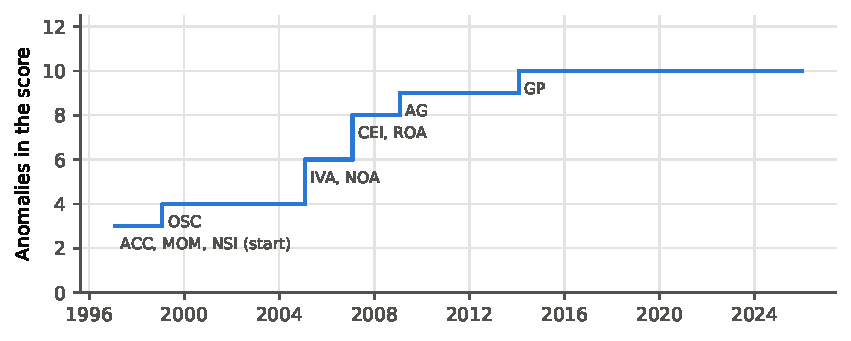
\includegraphics[width=0.92\textwidth]{../output/fig/fig1_entry.pdf}
\caption{Number of anomalies in the real-time score. Each anomaly enters in January of the year after its publication.}\label{fig:entry}\end{figure}

\begin{figure}[!htbp]\centering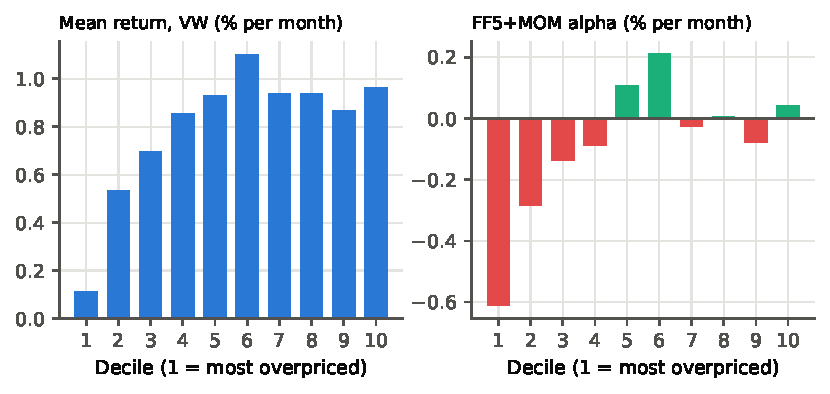
\includegraphics[width=0.92\textwidth]{../output/fig/fig2_deciles.pdf}
\caption{Decile portfolios of the real-time score, 1997--2025 (value-weighted, before costs): mean return and FF5+MOM alpha.}\label{fig:deciles}\end{figure}

\begin{figure}[!htbp]\centering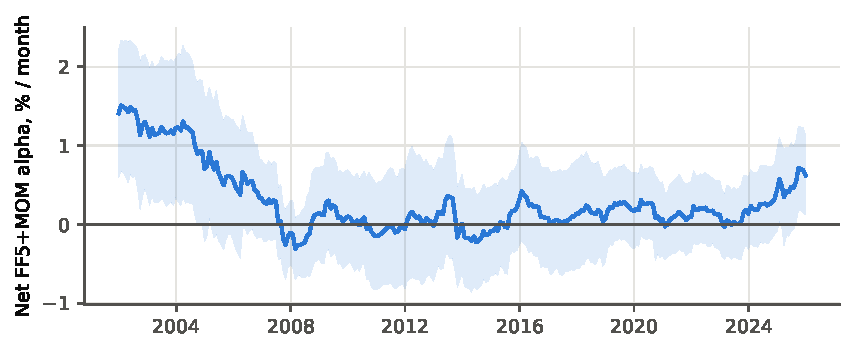
\includegraphics[width=0.92\textwidth]{../output/fig/fig4_rolling.pdf}
\caption{Rolling 60-month FF5+MOM alpha of the implementable strategy after costs, with 95\% confidence band (Newey--West).}\label{fig:rolling}\end{figure}

\begin{figure}[!htbp]\centering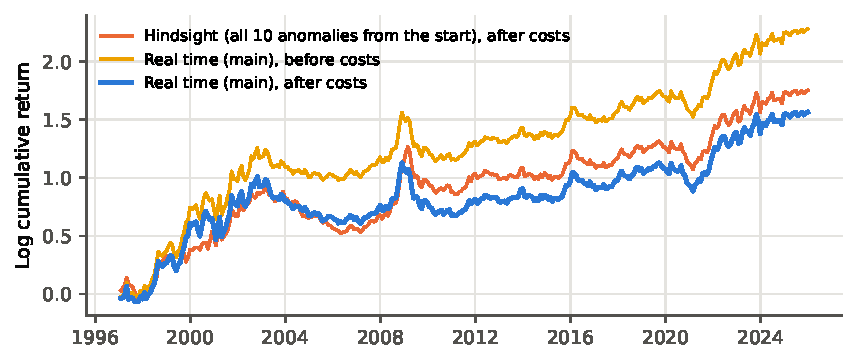
\includegraphics[width=0.92\textwidth]{../output/fig/fig5_versions.pdf}
\caption{Real time versus hindsight, and before versus after costs. Log cumulative long--short returns of the hindsight version after costs, and of the real-time strategy before and after costs.}\label{fig:versions}\end{figure}

\begin{figure}[!htbp]\centering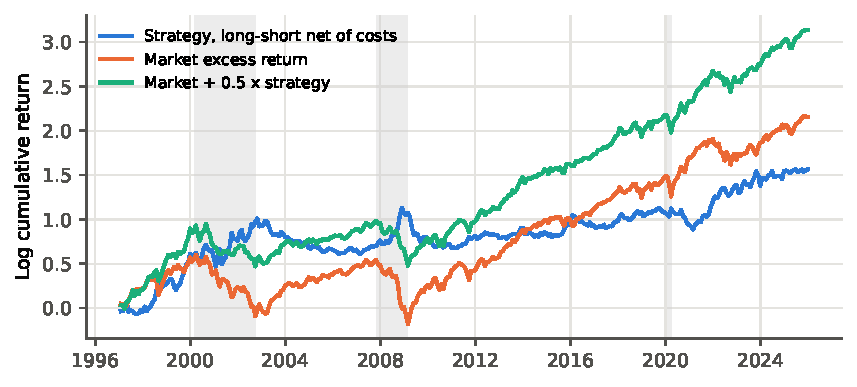
\includegraphics[width=0.92\textwidth]{../output/fig/fig3_cumulative.pdf}
\caption{Log cumulative returns, 1997--2025: the strategy after costs, the market excess return, and the market plus half a unit of the strategy.}\label{fig:cumulative}\end{figure}

\end{singlespace}
\end{document}
